\documentclass{standalone}
\usepackage{tikz}
\usepackage{float}
\usepackage{amsmath}
\usepackage{lmodern}
\usepackage{amssymb}
\usetikzlibrary{calc}
\usetikzlibrary{hobby}
\usepackage{nicefrac}
\usetikzlibrary{decorations.markings, decorations.pathreplacing}
\usetikzlibrary{patterns, patterns.meta}
\usetikzlibrary{shapes}
\usepackage{pgfplots}

\begin{document}

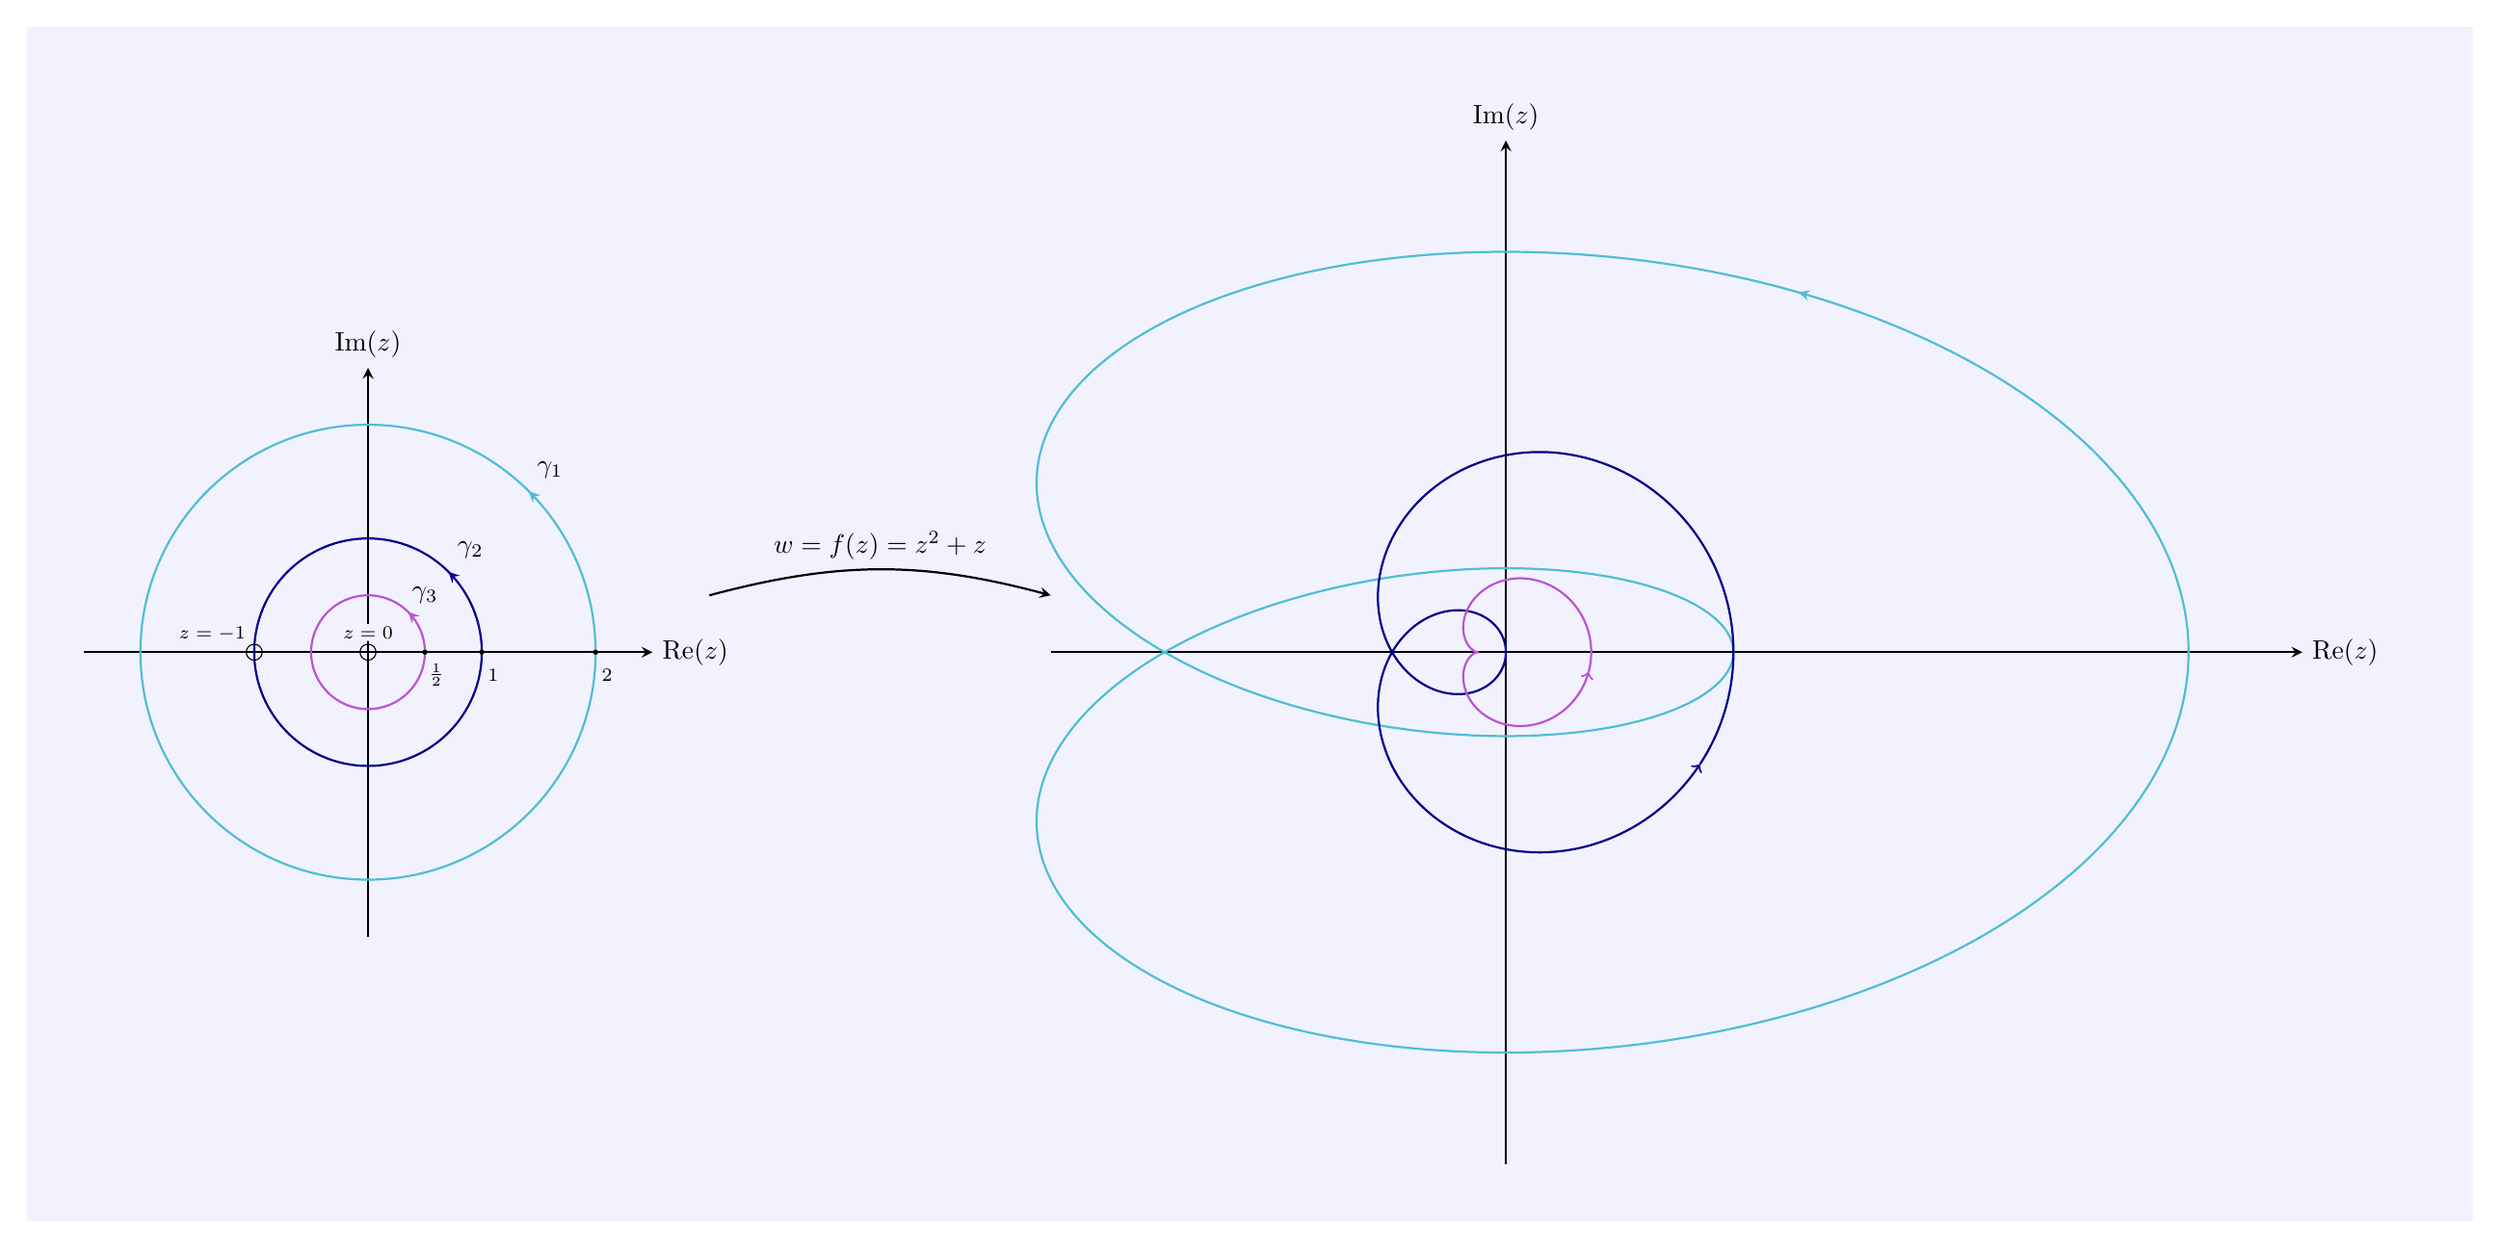
\begin{tikzpicture}[scale=1.5]

% Define the arrow decoration
\tikzset{
  arrow at angle/.style={
    postaction={
      decorate,
      decoration={
        markings,
        mark=at position #1 with {\arrow{stealth}}
      }
    }
  },
  arrowstyle/.style={->, >=stealth}
}

% Colors
\definecolor{gamma1}{RGB}{80, 190, 210}
\definecolor{gamma2}{RGB}{0,0,139}
\definecolor{gamma3}{RGB}{186,85,211}

% Background for entire canvas
\colorlet{BlueBackground}{blue!5}
\fill[BlueBackground] (-3,-5) rectangle (18.5,5.5);
    

\begin{scope}
  \draw[arrowstyle, thick] (-2.5,0) -- (2.5,0) node[right] {$\mathrm{Re}(z)$};
  \draw[arrowstyle, thick] (0,-2.5) -- (0,2.5) node[above] {$\mathrm{Im}(z)$};

  % Circles gamma1, gamma2, gamma3
  \draw[gamma1, thick, arrow at angle=0.125] (2,0) arc (0:360:2);
  \draw[gamma2, thick, arrow at angle=0.125] (1,0) arc (0:360:1);
  \draw[gamma3, thick, arrow at angle=0.125] (0.5,0) arc (0:360:0.5);

  % zeroes
  \newcommand{\DrawZero}[3]{%
    % function for drawing zeros
    % Inputs:
    % 1: coordinate (without parentheses, e.g. -1,0)
    % 2: label style
    % 3: label
    \node[solid, circle, draw=black, inner sep=0pt, minimum size=6pt] (ZeroCircle) at (#1) {};
    \node[#2,font=\scriptsize, inner sep=0pt] at (ZeroCircle) {#3};
  }

  \DrawZero{-1,0}{anchor=south east, xshift=-3pt, yshift=4pt}{$z=-1$}
  \DrawZero{0,0}{anchor=south, ellipse, fill=BlueBackground, yshift=4pt}{$z=0$}

  % Labels
  \node at (1.6,1.6) {$\gamma_1$};
  \node at (0.9,0.9) {$\gamma_2$};
  \node at (0.5,0.5) {$\gamma_3$};
  \node at (0.6,-0.2) {\scriptsize $\frac{1}{2}$};
  \node at (1.1,-0.2) {\scriptsize $1$};
  \node at (2.1,-0.2) {\scriptsize $2$};
  \filldraw[black] (0.5,0) circle (0.5pt);
  \filldraw[black] (1,0) circle (0.5pt);
  \filldraw[black] (2,0) circle (0.5pt);
\end{scope}

% Arrow and function label
\draw[arrowstyle, thick, bend left=15] (3,0.5) to node[midway, above] {$w = f(z) = z^2 + z$} (6,0.5);
    
% Right complex plane (w-plane)
\begin{scope}[shift={(10,0)}]
  \draw[arrowstyle, thick] (-4,0) -- (7,0) node[right] {$\mathrm{Re}(z)$};
  \draw[arrowstyle, thick] (0,-4.5) -- (0,4.5) node[above] {$\mathrm{Im}(z)$};

  % Parametric images of gamma1, gamma2, gamma3 under f(z) = z^2 + z
    \draw[domain=0:360,smooth,variable=\t,samples=400, gamma1, thick, arrow at angle=0.125]
    plot ({(2*cos(\t))^2 - (2*sin(\t))^2 + 2*cos(\t)},
          {2*(2*cos(\t))*(sin(\t)) + 2*sin(\t)});

  \draw[domain=-20:340,smooth,variable=\t,samples=400, gamma2, thick, ->]
    plot ({(cos(\t))^2 - (sin(\t))^2 + cos(\t)},
          {2*cos(\t)*sin(\t) + sin(\t)});

  \draw[domain=-10:350,smooth,variable=\t,samples=400, gamma3, thick,->]
    plot ({(0.5*cos(\t))^2 - (0.5*sin(\t))^2 + 0.5*cos(\t)},
          {2*(0.5*cos(\t))*(0.5*sin(\t)) + 0.5*sin(\t)});

\end{scope}

\end{tikzpicture}

\end{document}